\section{Introduction}

    \begin{wrapfigure}{r}{\textwidth/2}
        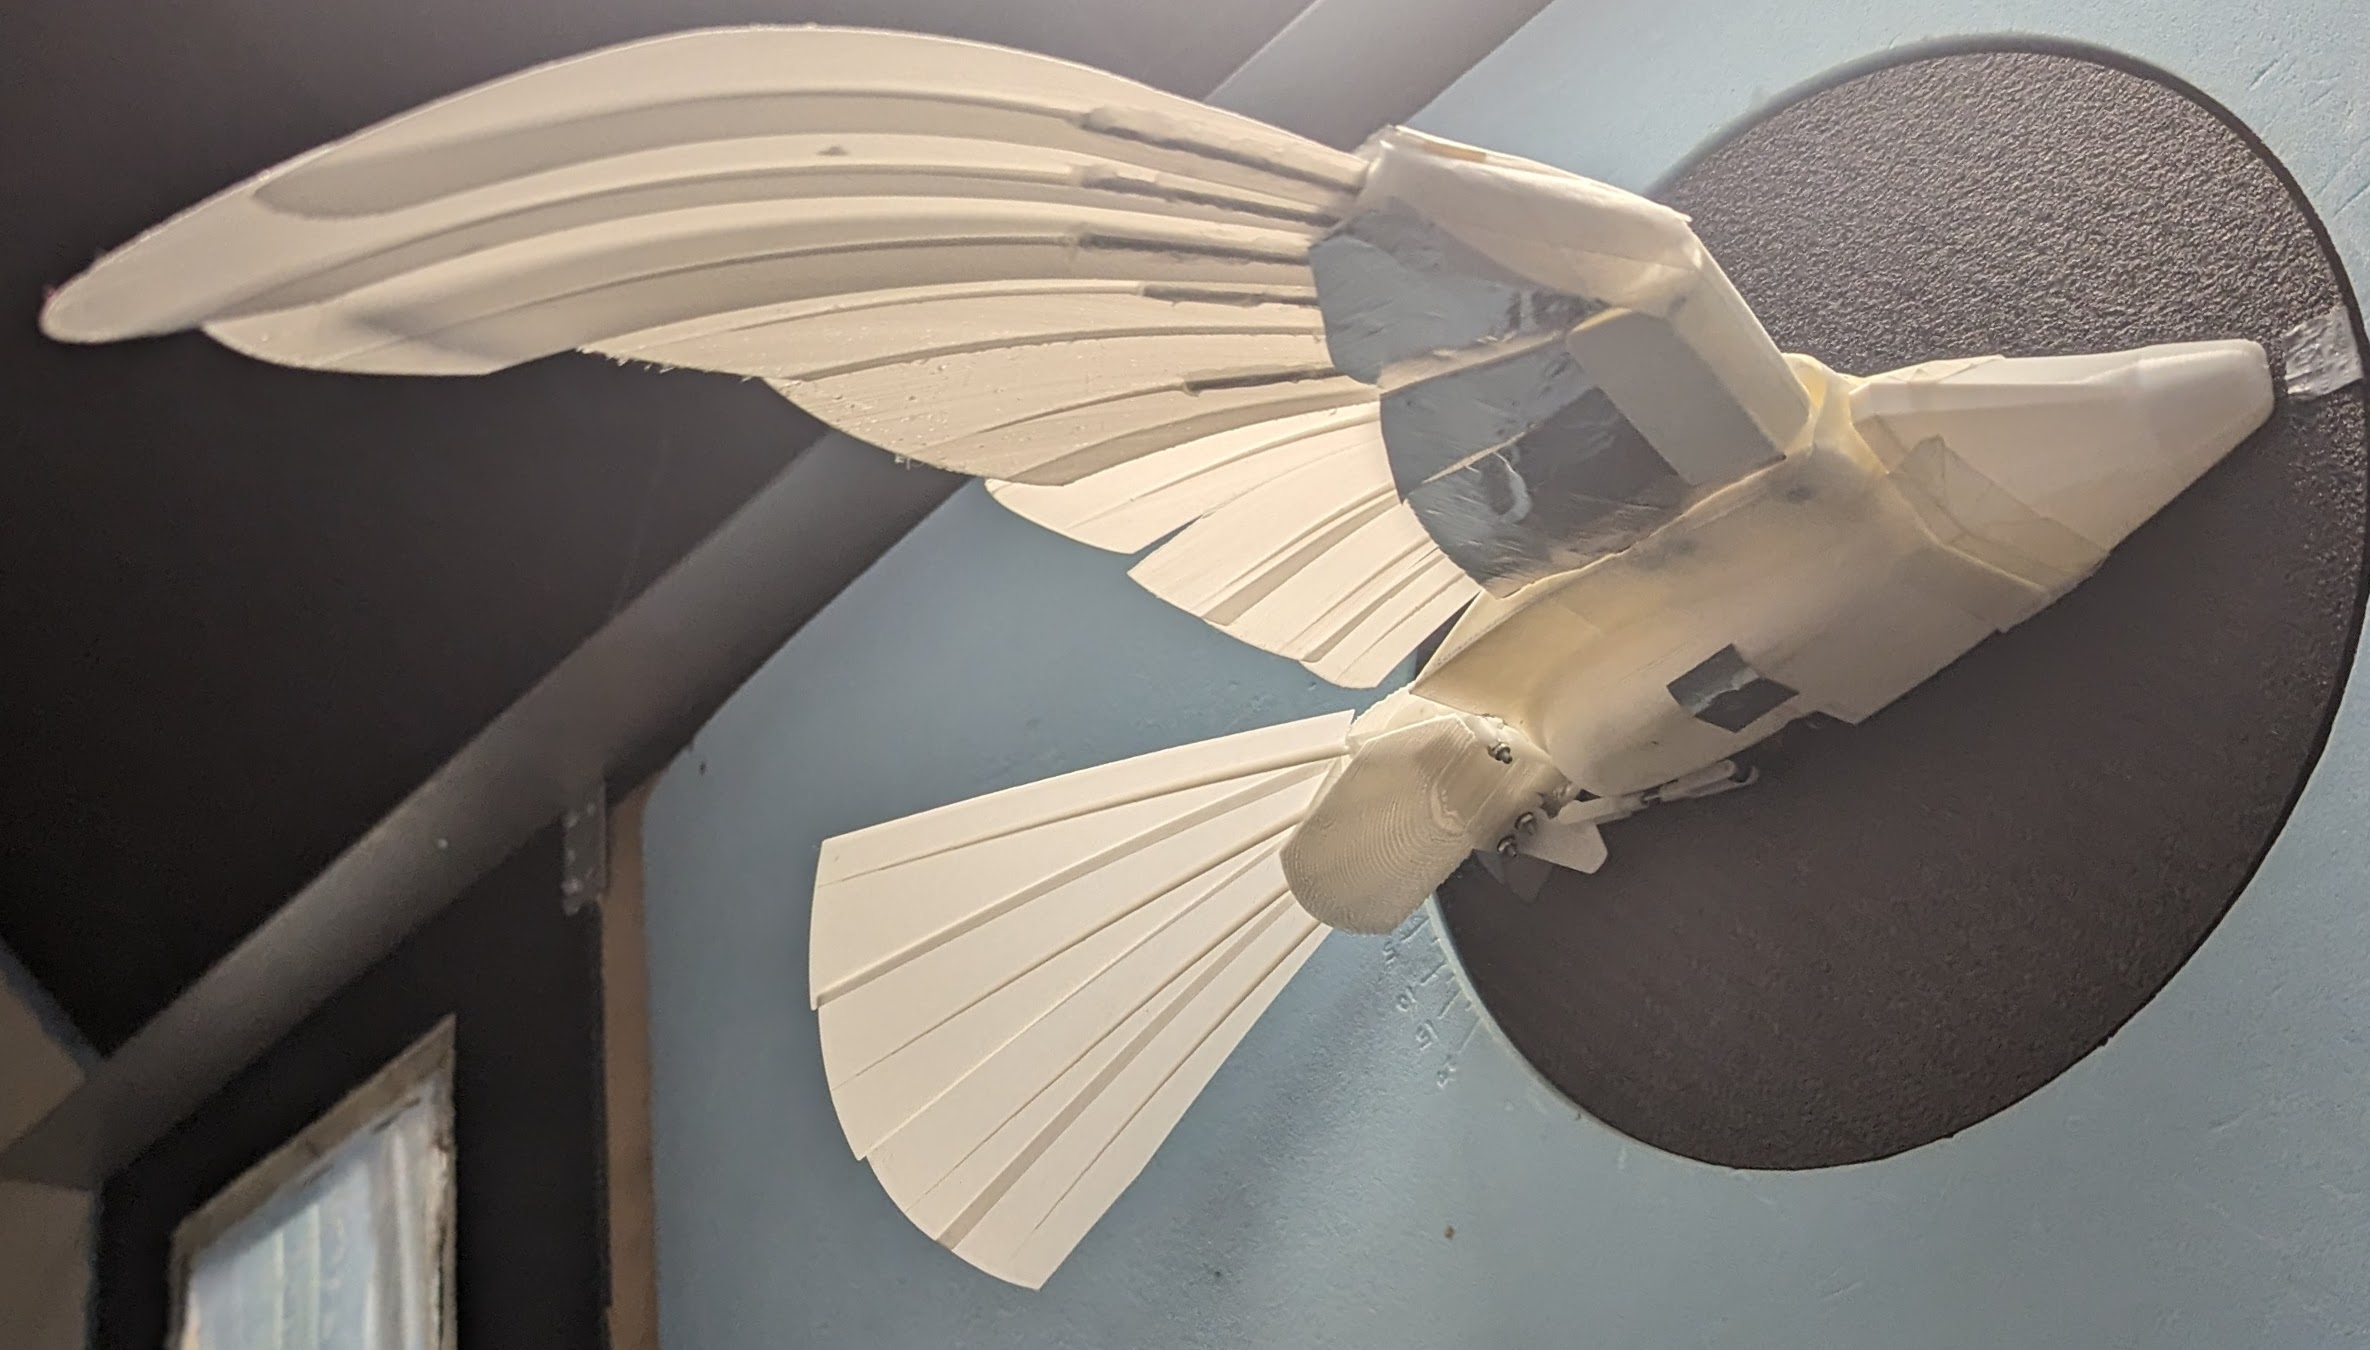
\includegraphics[width=\textwidth/2]{./img/Kestrel.jpg}
        \caption{\label{fig:figure 1} Kestrel Bird System}
    \end{wrapfigure}

    Mapping and surveying, environmental monitoring, delivery, search and
    rescue are some of the current applications of Unmanned Arial Vehicles
    (UAVs). Improving their ability to adjust to changes in wind conditions
    is a topic of much research \cite{1} especially as work continues to
    allow UAVs to carry out increasingly complicated tasks autonomously
    like CSIRO’s Hovermap an arial 3D mapping platform \cite{2}.

    In Australia the height limit to operate a UAV is 120m above ground
    level \cite{3}. At these heights wind turbulence and gust conditions greatly
    impact the performance of UAVs, by changing its trajectory and expected
    current state can potentially leading to drone damage. As a response to
    this, researchers have turned to nature as inspiration. Basing UAV
    design on birds has advantages over classical UAV designs (like
    multi-rotor or fixed wing drones) including increased aerodynamic
    efficiency, high manoeuvrability and stability in high-gust conditions \cite{4}.

    In this project we build on existing work to develop stable flight
    controllers for a novel platform the Kestrel robotic replica half-wing
    based on the Nankeen Kestrel with three degrees of freedom (wing
    extension, tail spread and tail pitch) \cite{5}
    (Figure 1).
    As a novel design
    the wing cannot be controlled with existing software, prior work on the
    Kestrel half-wing focussed on utilising Deep Reinforcement Learning
    (DRL) to develop a flight stability controller. DRL has been shown
    to have superior response time, reduced error and ability to reject
    external disturbances. Additionally, development of a DRL controller
    does not require domain specific knowledge in controller tuning \cite{6}.

    We will investigate the use of a classical controllers on the novel
    Kestrel platform to directly compare it to the DRL controller.
    We aim develop a Proportional Integral Derivative (PID) controller
    for flight stability already shown to be effective in stabilising UAVs
    \cite{7}.

\section{Related Work}
    PID control systems have been extensively explored in UAV
    stabilisation. According to a 2023 survey, Lopez-Sanchez et al.
    conducted an exhaustive literature review and realized that the most
    common control technique for quadrotor UAVs is PID control \cite{7}. With
    adaptive PID control being the most stable under unstable conditions,
    providing robustness against parameter uncertainty. An adaptive PID
    changes the gains of the controller during flight based on performance
    evaluation loop built into the controller. As all our testing will be
    conducted in laminar flow, an adaptive PID will not be implemented and a
    classical PID will be developed to reduce complexity of implementation.

    Tuning a PID using trial-and-error is a manual, tedious process often
    requiring expert domain knowledge \cite{6}. To address this, researchers are
    applying machine learning to the problem of finding high-performing gains
    for PID controllers. Support Vector Regression (SVR) is increasingly being
    used for PID controllers to facilitate the tuning process. Studies have
    shown that SVR-based controllers display enhanced stability and accuracy
    in variety of applications \cite{8}.

    In terms of applications in bio-inspired wings, Wenfu et al.\cite{9} in a 2021
    experiment showed the effectiveness of implementing a PID in a robotic
    bird. They describe that as their bird gets more complex, increasingly
    complex methods of control will be required. 

    As Okasha et al. discussed in their 2022 paper. Model Predictive Control
    (MPC) is a powerful controller that is more robust and stable compared
    to PID, though it is computationally expensive \cite{10}. Another advantage
    over PID is that it bypasses the tuning phase.

    The existing literature on PID, SVR tuning and MPC in the UAV space
    provided valuable insights for our project. By learning from these
    approaches, we can utilise a variety of control methods in a novel
    platform the Kestrel bio-inspired wing.

\section{Methodology}
    \subsection{System architecture}

	\begin{figure}[h]
	    \centering
    	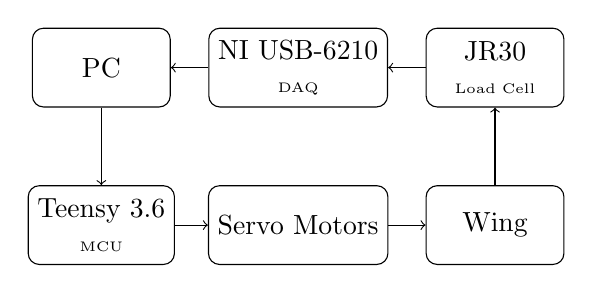
\begin{tikzpicture}
        	\tikzstyle{box} = [draw, rounded corners, minimum width=1.75cm, minimum height=1cm, align=center];
        	\node[box] (PC) {PC};
            \node[box, below of=PC, yshift=-1cm] (MCU) {Teensy 3.6\\\tiny MCU};
        	\node[box, right of=MCU, xshift=1.5cm] (servo) {Servo Motors};
        	\node[box, right of=servo, xshift=1.5cm] (wing) {Wing};
        	\node[box, above of=wing, yshift=1cm] (load) {JR30\\\tiny Load Cell};
        	\node[box, left of=load, xshift=-1.5cm] (DAQ) {NI USB-6210\\\tiny DAQ};

            \draw[->] (PC) -- (MCU);
            \draw[->] (MCU) -- (servo);
            \draw[->] (servo) -- (wing);
            \draw[->] (wing) -- (load);
            \draw[->] (DAQ) -- (PC);
            \draw[->] (load) -- (DAQ);
    	\end{tikzpicture}
        \caption{Experimental system architecture}\label{fig:architecture_hardware}
	\end{figure}

	Figure~\ref{fig:architecture_hardware} outlines the experimental setup from a hardware perspective, where notably a circular feedback system is implemented. The wing connects to a JR30 load cell mounted internal to the wind tunnel. This load cell is connected via DB9 connector to a data acquisition box (DAQ) which in turn wires a USB connection into the computer to interface with the controller software.

	Data is collected from the DAQ through the \verb|NI-DAQmx| driver software. As discussed further in this report, the DAQ \textit{must} be calibrated before use to ensure output measurements are correct and nominal. Once the load feedback from the wing is processed by the controller, outputs are generated for each of the three servos controlling the respective wing extension, tail spread, and tail pitch of the model. These then pass to the \verb|Teensy| microcontroller (MCU) over serial communication via USB. 

    \vspace{-1em}
    \begin{wrapfigure}{l}{0.5\textwidth}
        \begin{center}
            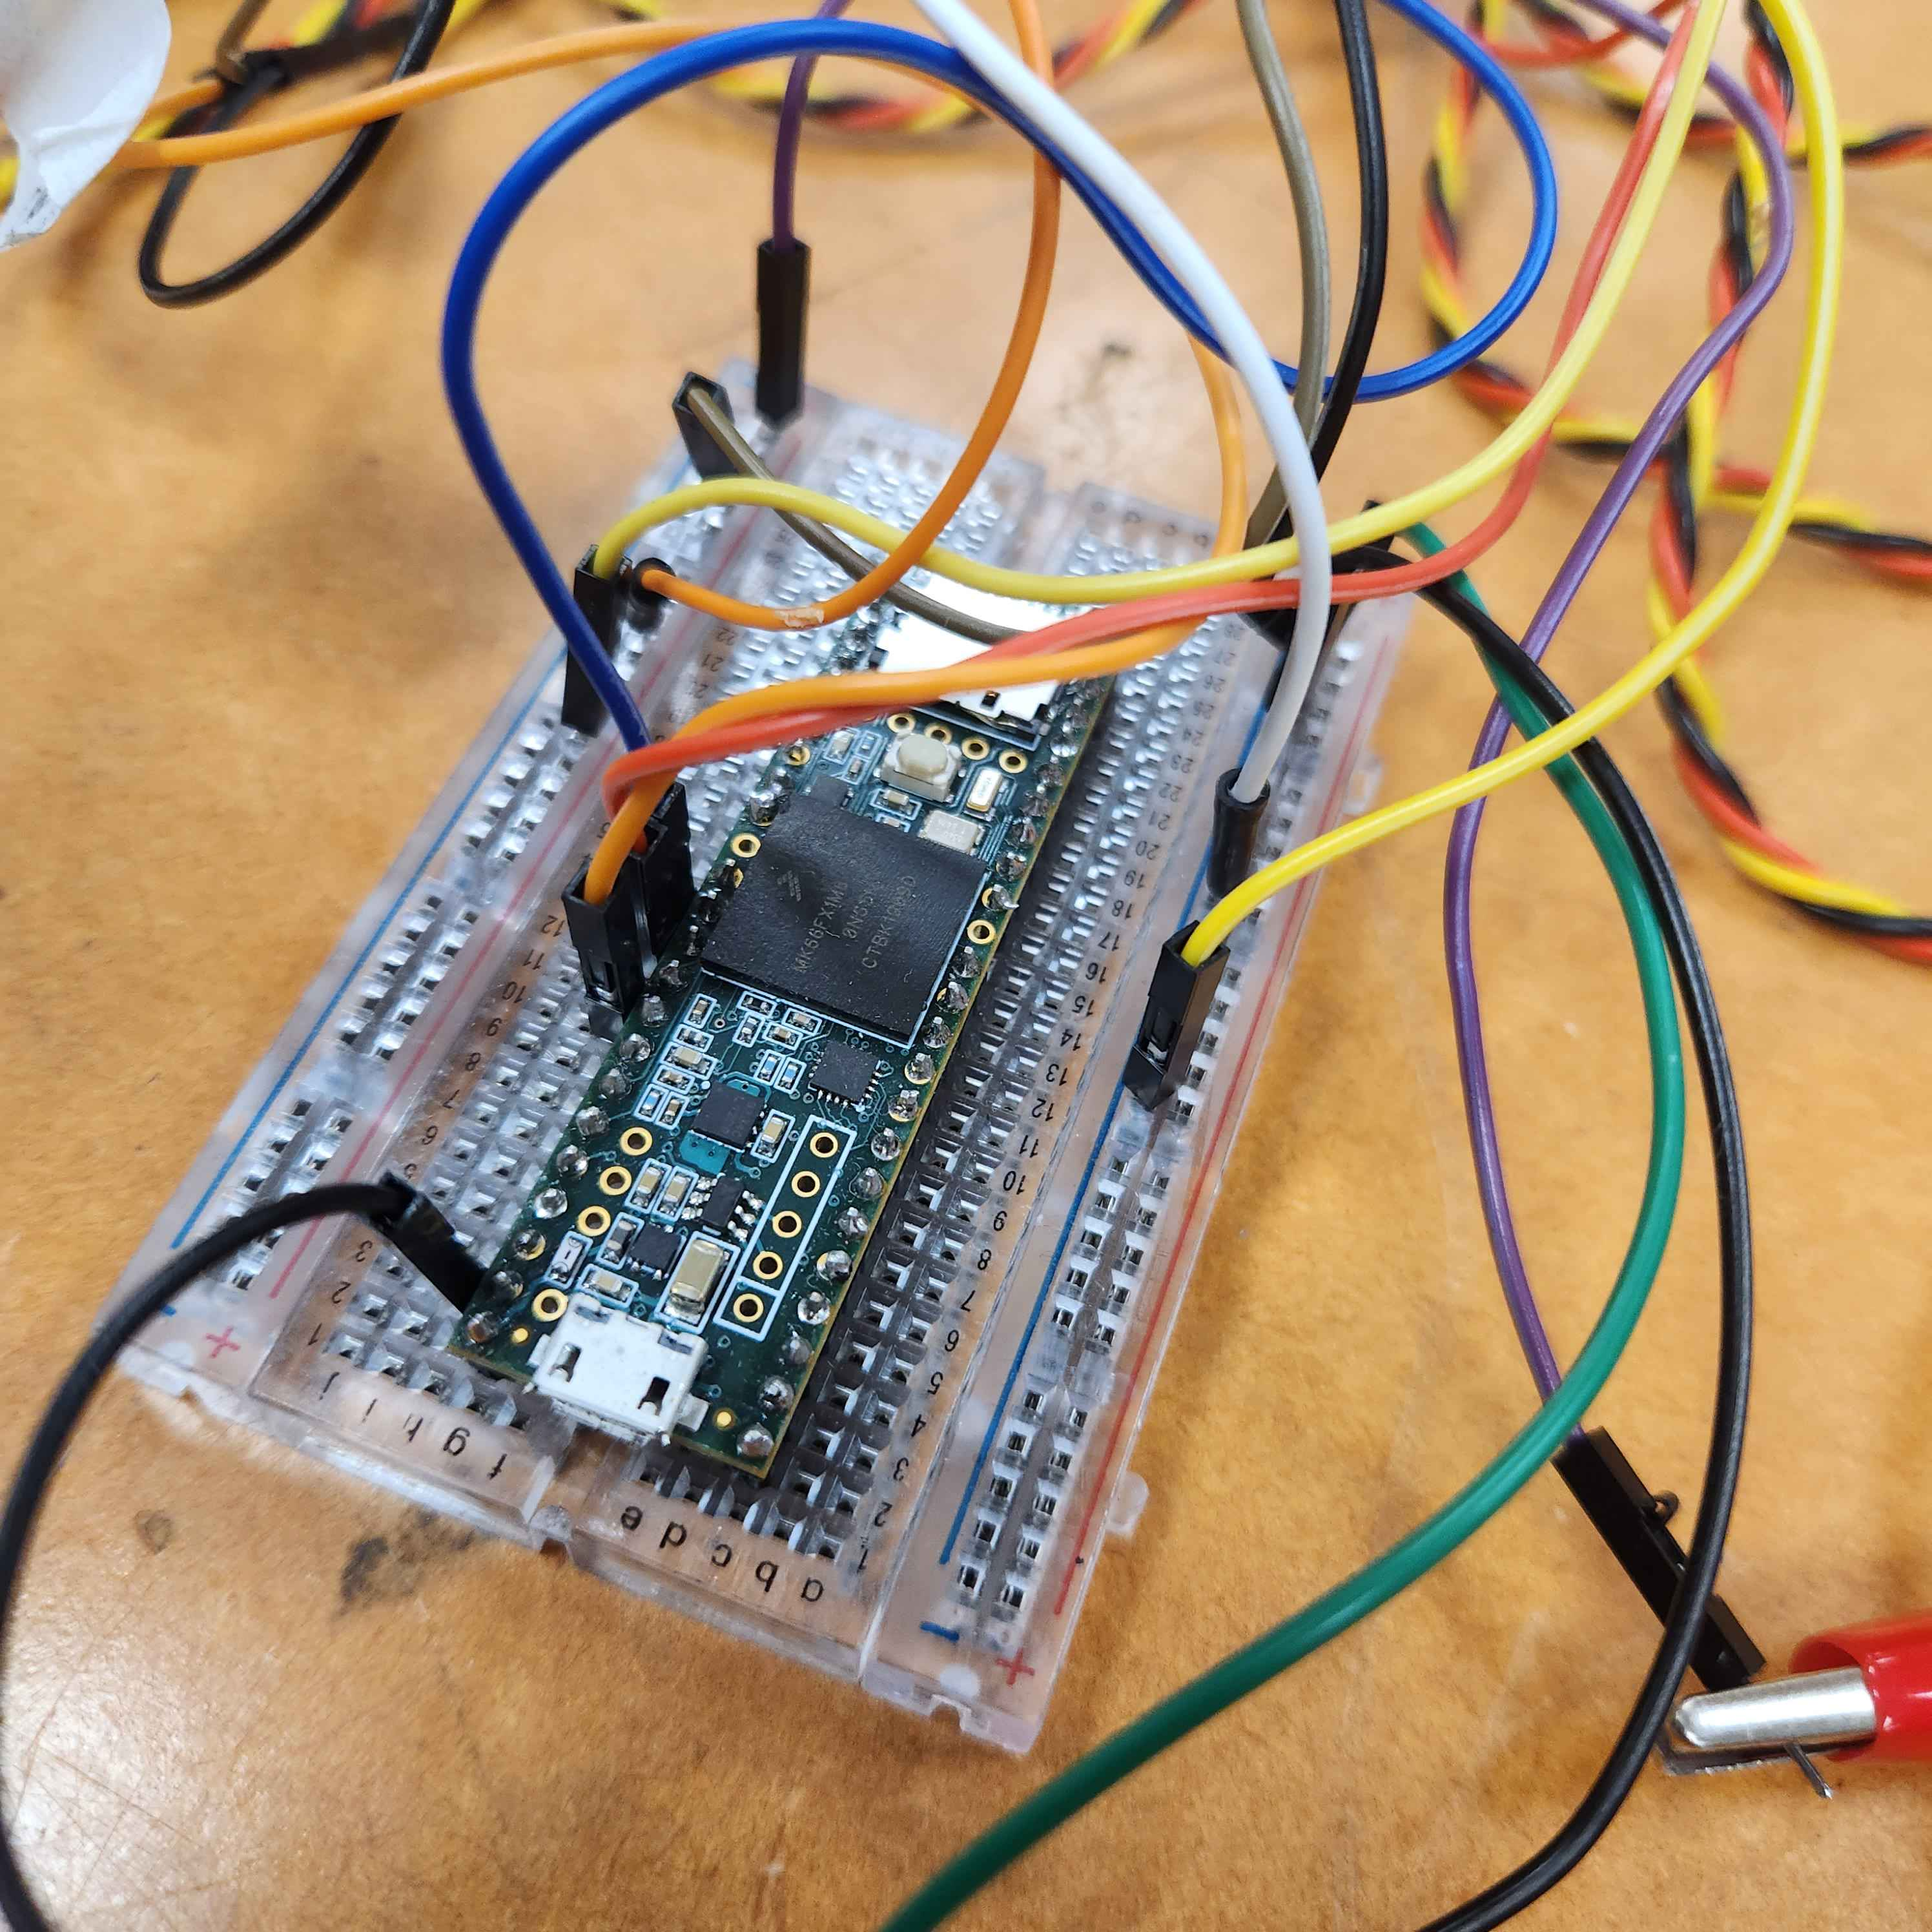
\includegraphics[width=0.45\textwidth]{./img/hardware_breadboard.jpg}
        \end{center}
        \caption{Breadboard setup for Teensy microcontroller}\label{fig:hardware_breadboard}
    \end{wrapfigure}

	Internally, the MCU firmware handles the hardware interfacing with the servos to drive the wing, moving to the pose as determined by the controller. 

    \subsection{Software architecture}
	\begin{wrapfigure}{r}{\textwidth/3}
    	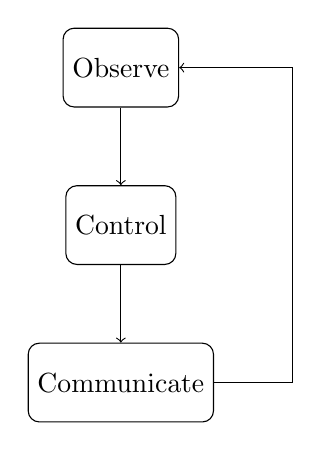
\begin{tikzpicture}[scale=1]

        	\tikzstyle{box} = [draw, rounded corners, minimum width=1cm, minimum height=1cm, align=center];

        	\node[box] (tier3) {Observe};
        	\node[box, below of=tier3, node distance=2cm] (tier2) {Control};
        	\node[box, below of=tier2, node distance=2cm] (tier1) {Communicate};

        	\draw[->] (tier3) -- (tier2);
        	\draw[->] (tier2) -- (tier1);
        	\draw[->] (tier1.east) -- ++(1cm,0) arc (0:0:2cm) |- (tier3.east);

    	\end{tikzpicture}
        \caption{Software architecture}\label{fig:architecture_software}
	\end{wrapfigure}

    For our software system, we developed an N-tier software architecture.
    Our architecture contains 3 main tiers, as outlined in Figure~\ref{fig:architecture_software}.

    Firstly we have the observation
    tier, which links into the Kestrel’s observation space, this includes
    the Kestrel’s motor positions and collects data from the load cell that
    the bird is plugged into.

    Secondly is the controller layer, being a
    component layer that allows us to plug in any of our developed controllers
    either the PID or the MPC controller this layer also includes the training
    of these controllers for example with the PID controller the SVR Tuner we
    have developed also runs with the data collected from the observation tier.

    \begin{figure}[h]
        \begin{center}
            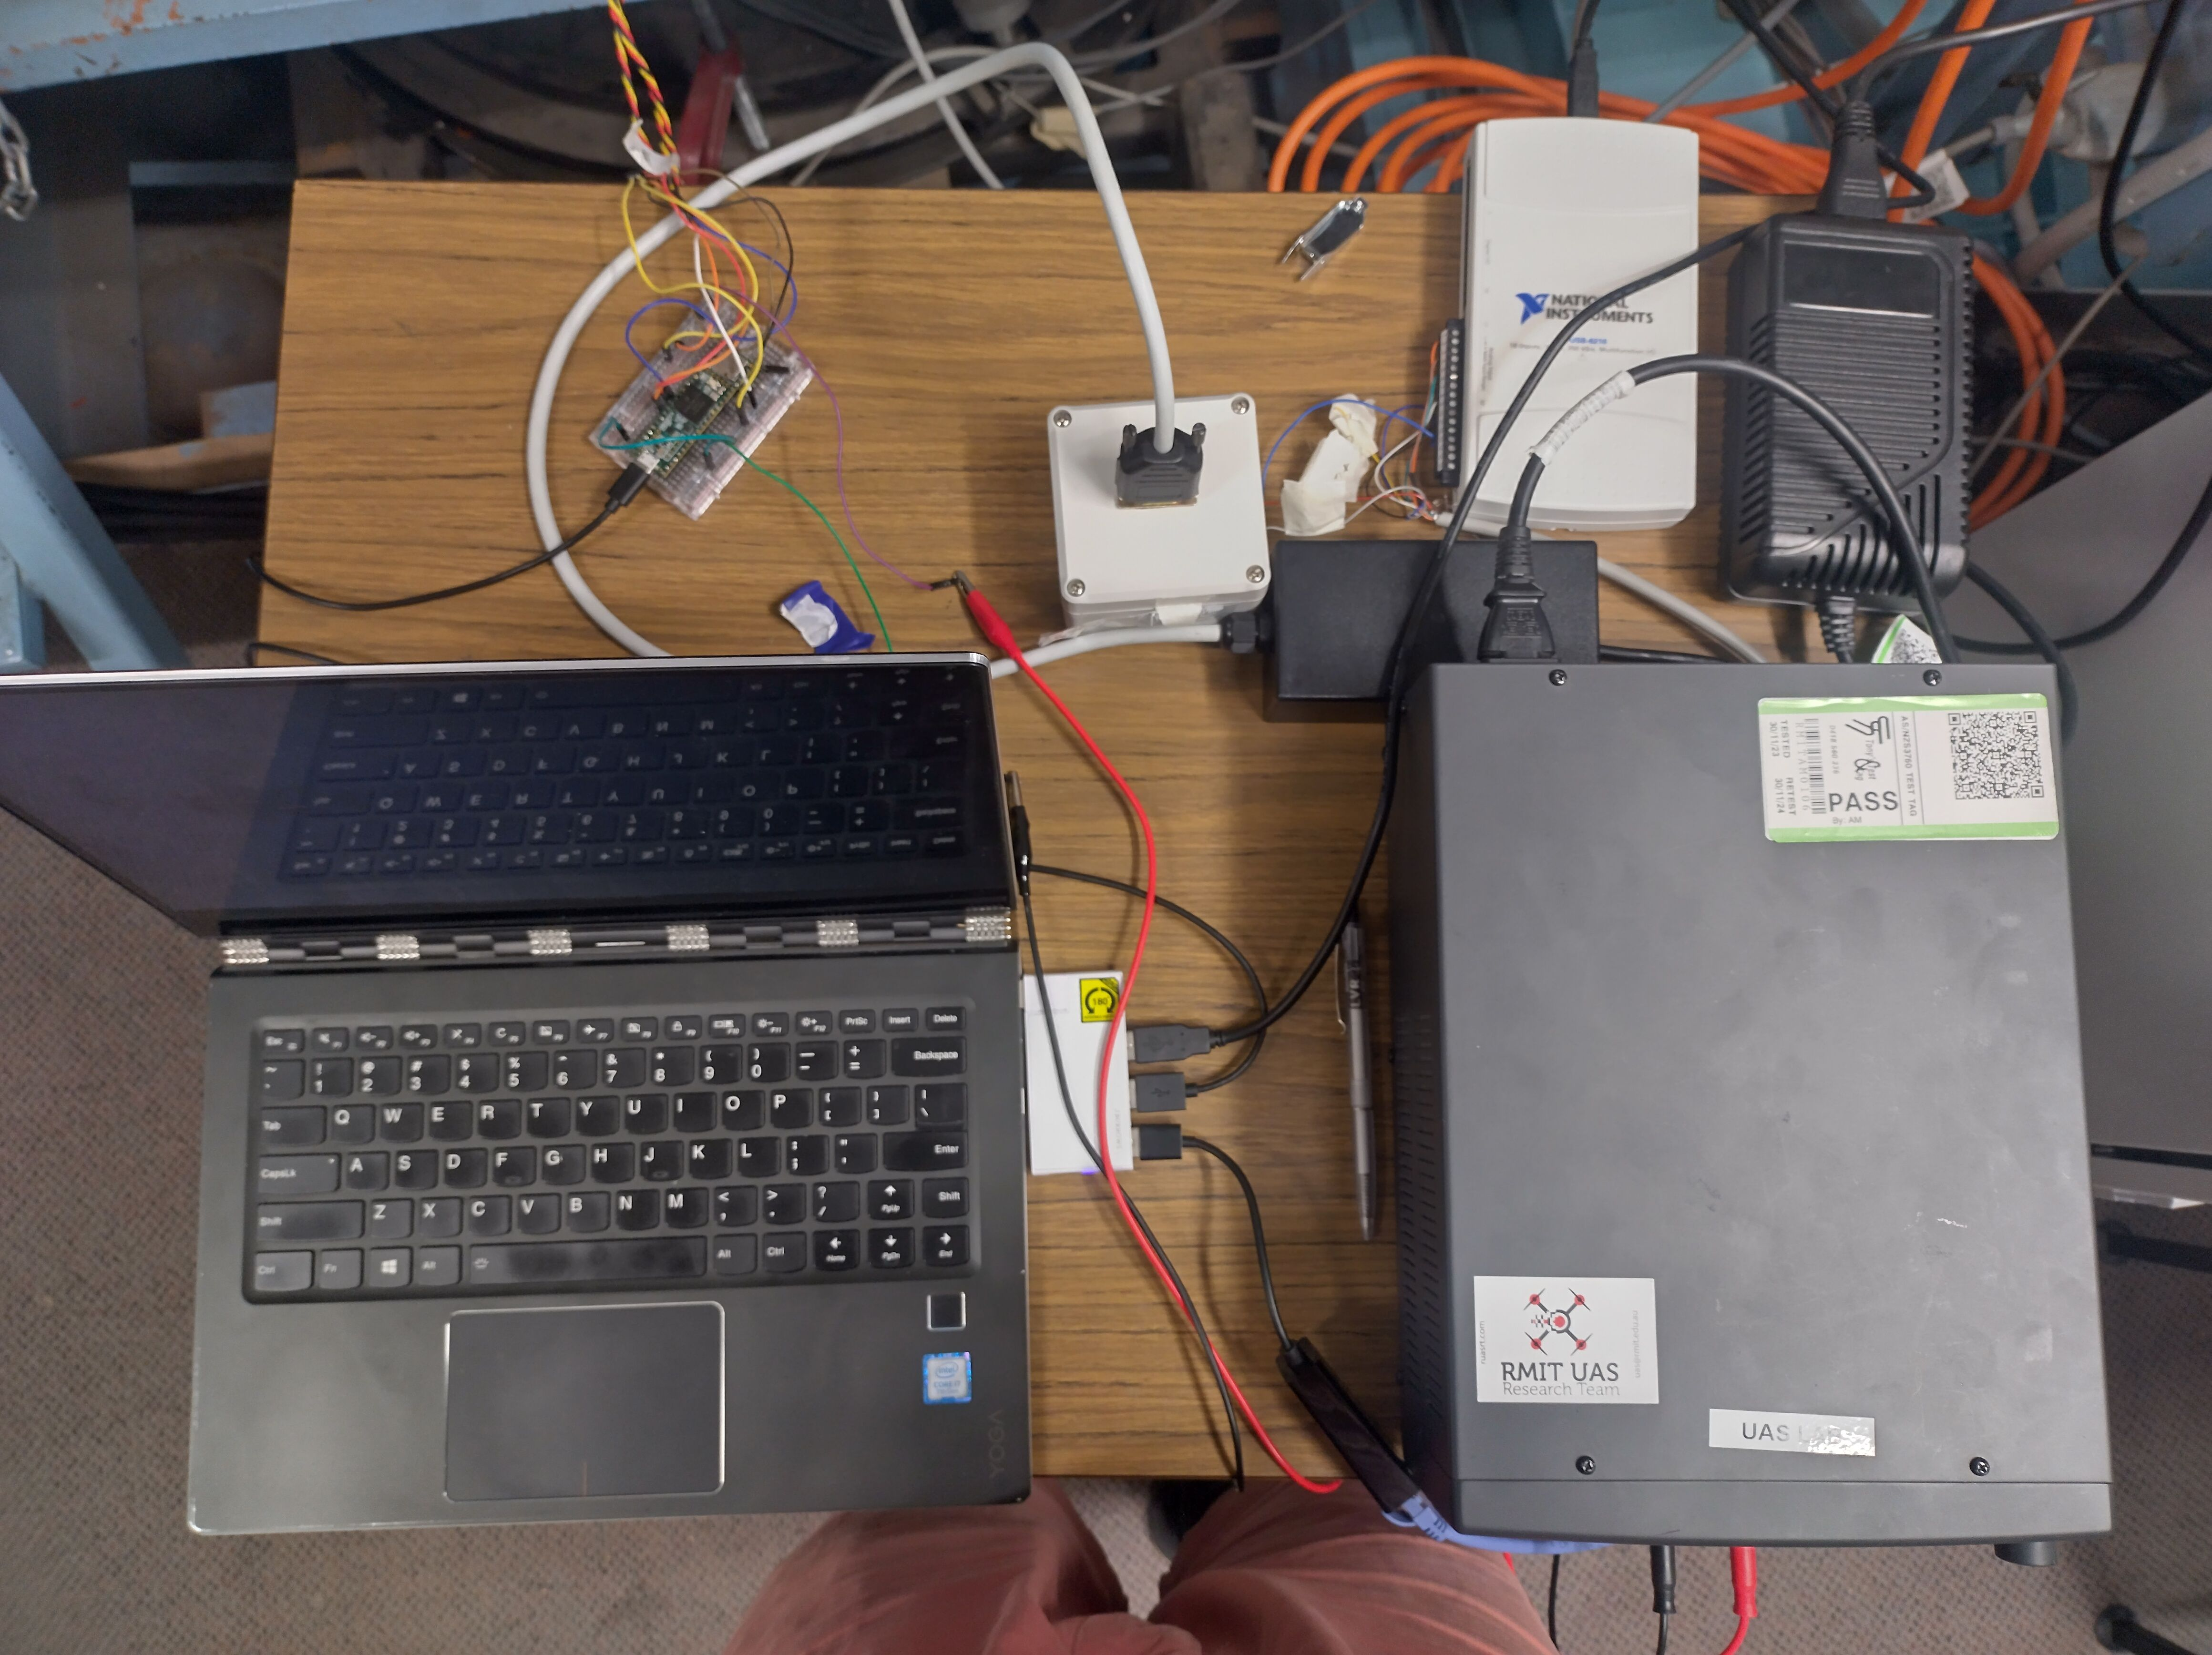
\includegraphics[width=0.7\textwidth]{./img/hardware_setup.jpeg}
        \end{center}
        \caption{System hardware setup}\label{fig:hardware_setup}
    \end{figure}

    
    Finally, we have the Communication tier, which takes the place of the
    presentation layer. This takes everything that the previous tiers have done
    and sends the data to the Kestrel’s action space, this then finally loops
    back to the observation tier to do it all again.

    \subsection{Developed Software}

    \paragraph{PID controller} Firstly we developed a generic PID
    controller as a method of controlling the Kestrel bird. The PID
    controller takes in an initial P, I, and D value to dictate the
    controller's response, as well as a setpoint which is a targeted
    system value. For the PID controller to operate effectively the
    P, I and D values need to be optimally selected and for this, we
    move on to the next piece of software.
    
    \paragraph{SVR Tuner} We developed the SVR Tuner as a modern method
    of selecting the most optimal P, I, and D values for the PID controller,
    we chose this regressional method based on the identifiable success that
    others have had in similar applications \cite{12}. Our tuning is split into
    several episodes. For each episode, the tuner goes through an exploration
    phase to build up the data for the tuner to work with and all this data
    is then collected and processed to find the best PID values for our controller.

    \paragraph{MPC} We have also implemented a Model Predictive Controller, though
    due to the relative complexity of the algorithm, we have opted to implement a
    pre-existing library \href{https://github.com/forgi86/pyMPC}{pyMPC} which was selected due to its simplicity and the 
    overall control we have over the setup. We chose this to compare directly
    against the PID controller, MPC by design is a predictive controller
    whereas PID is reactive, which gives us a good benchmark for the control
    system of the bird.

    \clearpage
    \subsection{Experiment details}
    \setlength{\intextsep}{0pt}
    \begin{wrapfigure}{r}{\textwidth/2}
        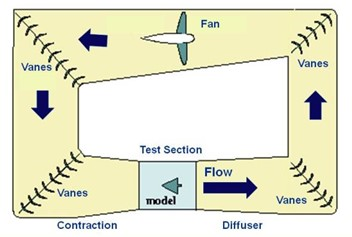
\includegraphics[width=\textwidth/2]{./img/Fig2_wind_tunnel_design.jpg}
        \caption{\label{fig:figure 2} Closed Return Wind Tunnel \cite{10}}
    \end{wrapfigure}
    \paragraph{Wind tunnel}
    The Kestrel will be mounted in the blue wind tunnel at the RMIT
    Bundoora Campus. It is a closed return wind tunnel \cite{11}. The
    wind tunnel is built across two floors with wind generated by a fan on
    the first floor sent to the second floor where the testing area is.
    This design ensures steady delivery of laminar flow, wind flow without
    disturbances. Figure 2 from displays this generic design. The vanes on
    each corner of the tunnel ensure that the flow is laminar. 

    A pressure probe embedded in the test area allows us to assess the
    pressure in the wind tunnel. Knowing the target speed and the ambient
    temperature and air pressure of the wind tunnel allows us to calculate
    a target pressure which is what we aim for when testing. All our testing
    occurred at approximately 0.0155 kPa or 5 m/s, the target pressure would
    fluctuate throughout the day as ambient temperature and pressures
    changed. As such we regularly calculated the target pressure to ensure
    consistent speeds.

    \begin{wrapfigure}{r}{\textwidth/2}
        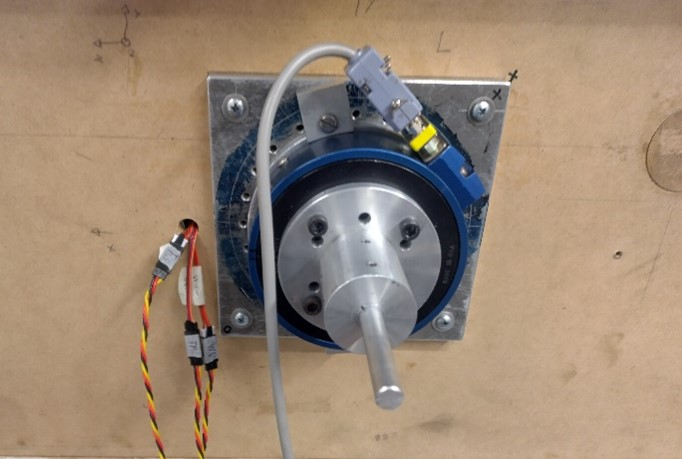
\includegraphics[width=\textwidth/2]{./img/Fig3_load_cell.jpg}
        \caption{\label{fig:figure 3} 30N Load Cell}
    \end{wrapfigure}

   \paragraph{Load cell} The Kestrel is mounted directly onto a 30 N load cell (Figure 3). The
   output from the load cell describes the major forces occurring on the
   Kestrel. After processing through the data acquisition box, we are given
   a list of 6 values: the force in N at X, Y and Z. We are also given
   moments in X, Y and Z, which is expressed in Nm. The primary force used
    in training and testing was the force at Y or the lift.

    Before each test the load cell must be calibrated to ensure we return
    accurate results. In our design we take 1000 results from the load cell
    and store the average for each measure in a file. This average is then
    subtracted from each test measurement to zero the load cell. We recognised
    some drift in the load cell and therefor we calibrated the load cell regularly.

    \paragraph{Data output}
    After a test everything that happens at each timestep this includes all the
    forces in N and moments in Nm, the new set position of each servo as decided by
    the controller and the error lift. For all tests the lift of the bird was
    targeted to be 0.42 N. This data will be sufficient to capture our primary outcomes:

    \begin{itemize}
        \item Time taken to stabilise the bird
        \item Quality of transition to stability
        \item Quality of stability (error is as close to zero as possible throughout flight)
    \end{itemize}

    \paragraph{Experimental design} In addition to assessing the robustness of our controllers the output will
    allow us to compare to the pre-trained DRL model.
    The following is the experimental workflow that was carried out to conduct each major test.

    \begin{enumerate}
        \item Load cell calibration, to zero the load cell
        \item Dynamic pressure assessment, to ensure consistent speeds
        \item Set wind speed, based on dynamic pressure assessment
        \item Run test of interest PID / MPC / SVR tuner
        \item Data collection
    \end{enumerate}

\section{Results}

\begin{figure}[h!]
    \centering
    \begin{subfigure}[b]{0.49\textwidth}
        \centering
        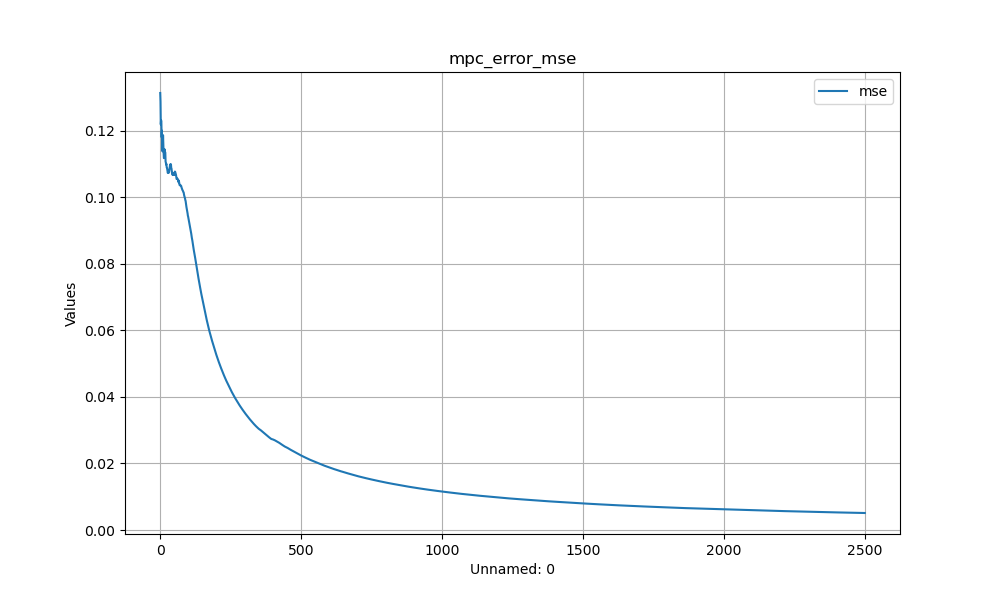
\includegraphics[width=\textwidth]{./img/mpc_error_mse.png}
        \caption{MPC error at -5\textdegree\ }
    \end{subfigure}
    \begin{subfigure}[b]{0.49\textwidth}
        \centering
        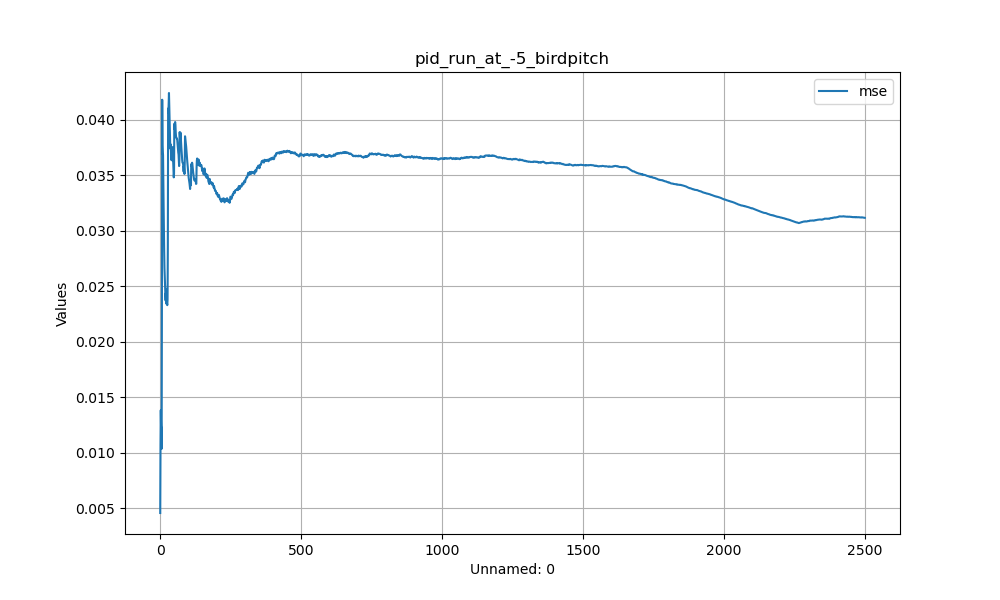
\includegraphics[width=\textwidth]{./img/pid_run_at_-5_birdpitch.png}
    \caption{PID error at -5\textdegree\ pitch}
    \end{subfigure}
    \begin{subfigure}[b]{0.49\textwidth}
        \centering
        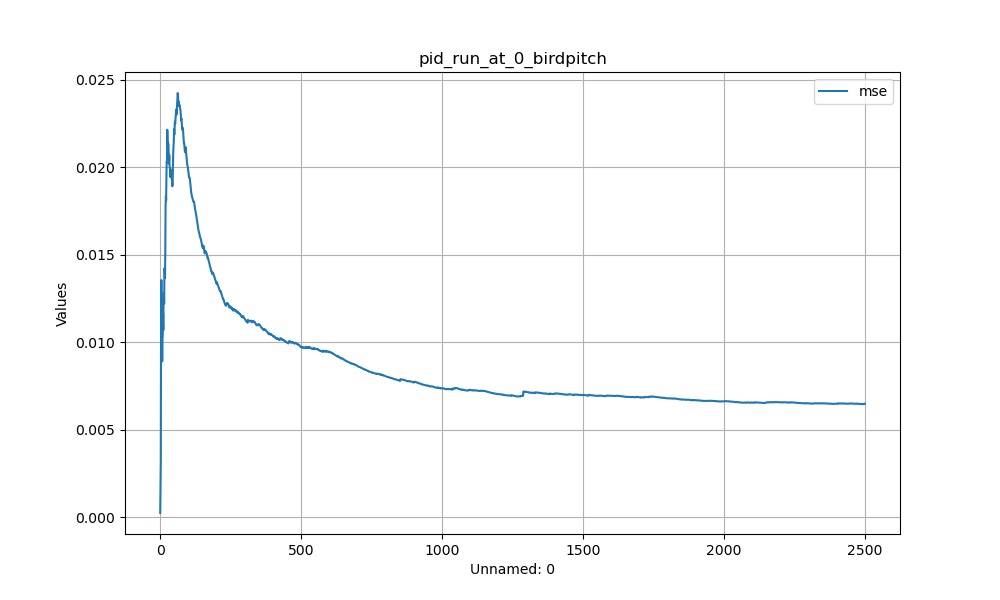
\includegraphics[width=\textwidth]{./img/pid_run_at_0_birdpitch.png}
        \caption{PID error at 0\textdegree\ pitch}
    \end{subfigure}
    \begin{subfigure}[b]{0.49\textwidth}
        \centering
        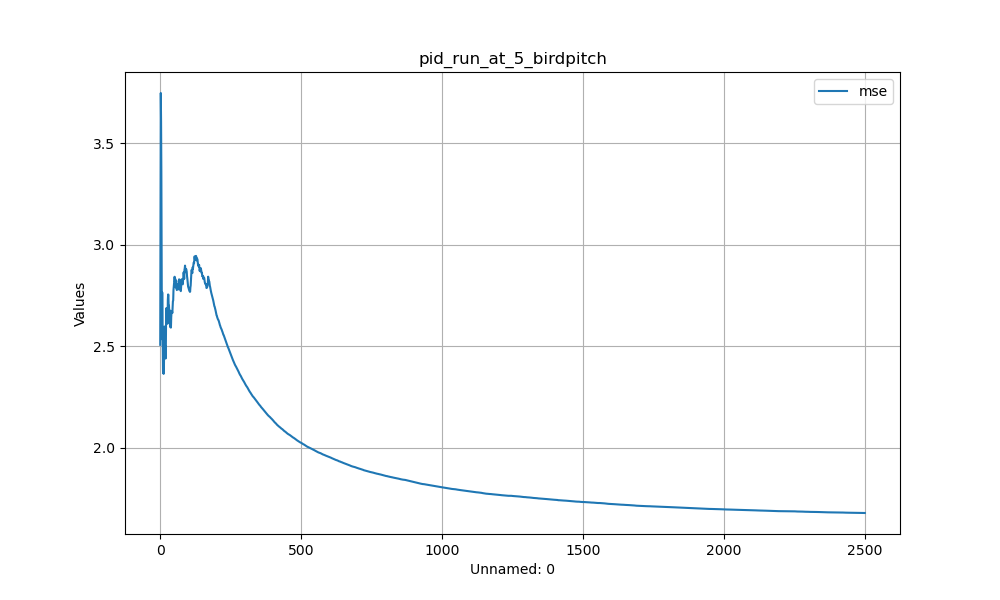
\includegraphics[width=\textwidth]{./img/pid_run_at_5_birdpitch.png}
        \caption{PID error at 5\textdegree\ pitch}
    \end{subfigure}
    \caption{Evaluation runs of the 2 controllers}
    \label{fig:four_images}
\end{figure}

    Here we have the final runs of our controllers firstly to the top right
    we have the MPC run, due to time constraints we were only able to get a
    full test of the MPC controller running at -5\textdegree{} but from the
    graph we can see that the controller was able to begin stabilizing at
    approx 500 timesteps and by 1000 timesteps the controller has fully
    stabilized this is significant due to the controller not requiring a
    dedicated training phase.


    Now we have the PID controller, the controller with the optimal
    settings managed to stabilize very quickly at both 0\textdegree{}
    and 5\textdegree{} pitches but seemed to not move very much at the
    -5\textdegree{} pitch.


    We can also take a look at the final positions of the bird at the
    end of each run. The MPC controller had the Wing spread and the Tail
    spread at very similar levels ranging from about -9.3 to -9.7 and having
    the Tail pitch at about 0.57.

    The pid runs are quite different from this, for -5\textdegree{} has all the
    positions negative with both of the tail positions at -1 and the wing spread
    at -0.2 but then if we move on to 0\textdegree{} we have all of the servo
    positions at 1 and at 5\textdegree{} all of the servo positions at -1 this
    could suggest many things such as the bird not physically being able to get
    to the target load at some of the sharper pitches.

    \vspace{0.25em}\noindent Video recordings of the PID runs are available via the following links:
    \begin{itemize}
        \item \href{https://www.dropbox.com/scl/fo/qydc6hqrx3budknwzgmi1/ADdN0YC3AZ4ctg0SImbJqqI/Videos?preview=final_PID_0.mp4&rlkey=jcnhrcvje207wu5aaq48laen6&subfolder_nav_tracking=1&st=k76cp6vc&dl=0}{\color{blue}\underline{PID 0\textdegree{} run}}
        \item \href{https://www.dropbox.com/scl/fo/qydc6hqrx3budknwzgmi1/ADdN0YC3AZ4ctg0SImbJqqI/Videos?preview=final_PID_neg5.mp4&rlkey=jcnhrcvje207wu5aaq48laen6&subfolder_nav_tracking=1&st=log0nht8&dl=0}{\color{blue}\underline{PID -5\textdegree{} run}}
        \item \href{https://www.dropbox.com/scl/fo/qydc6hqrx3budknwzgmi1/ADdN0YC3AZ4ctg0SImbJqqI/Videos?preview=final_PID_0.mp4&rlkey=jcnhrcvje207wu5aaq48laen6&subfolder_nav_tracking=1&st=k76cp6vc&dl=0}{\color{blue}\underline{PID 5\textdegree{} run}}
    \end{itemize}

\section{Evaluation}

\begin{figure}[h]
    \centering
    \begin{subfigure}[b]{0.49\textwidth}
        \centering
        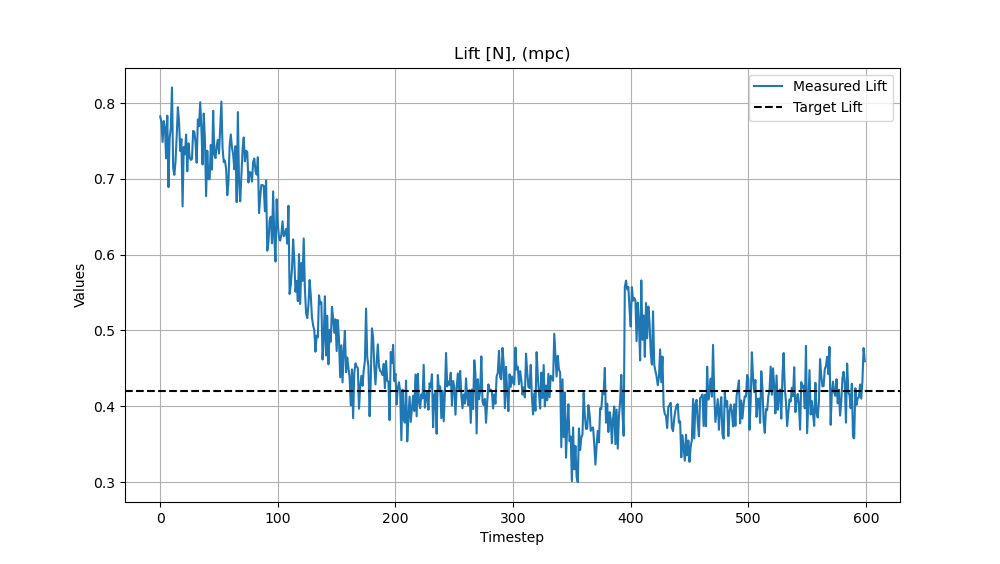
\includegraphics[width=\textwidth]{./img/LiftMPC.png}
        \caption{MPC at $\SI{-5}{\degree}$}
    \end{subfigure}
    \begin{subfigure}[b]{0.49\textwidth}
        \centering
        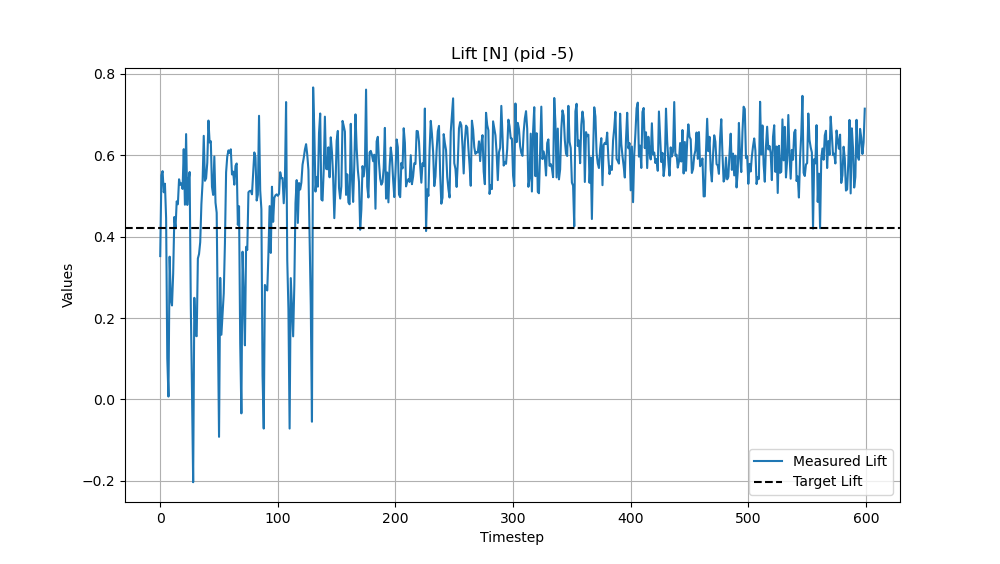
\includegraphics[width=\textwidth]{./img/LiftPID-5.png}
        \caption{PID at $\SI{-5}{\degree}$}
    \end{subfigure}
    \begin{subfigure}[b]{0.49\textwidth}
        \centering
        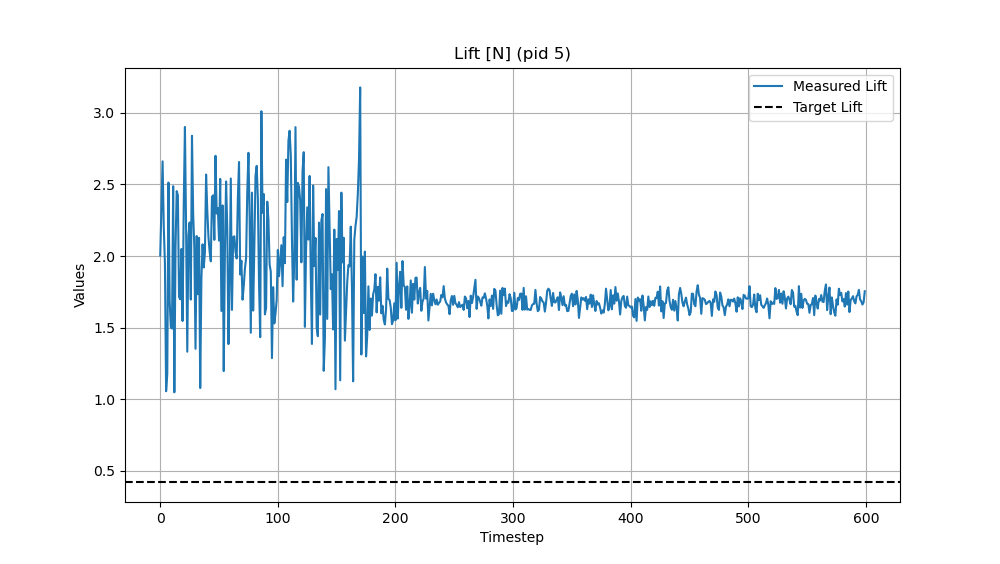
\includegraphics[width=\textwidth]{./img/LiftPID5.png}
        \caption{PID at $\SI{5}{\degree}$}
    \end{subfigure}
    \begin{subfigure}[b]{0.49\textwidth}
        \centering
        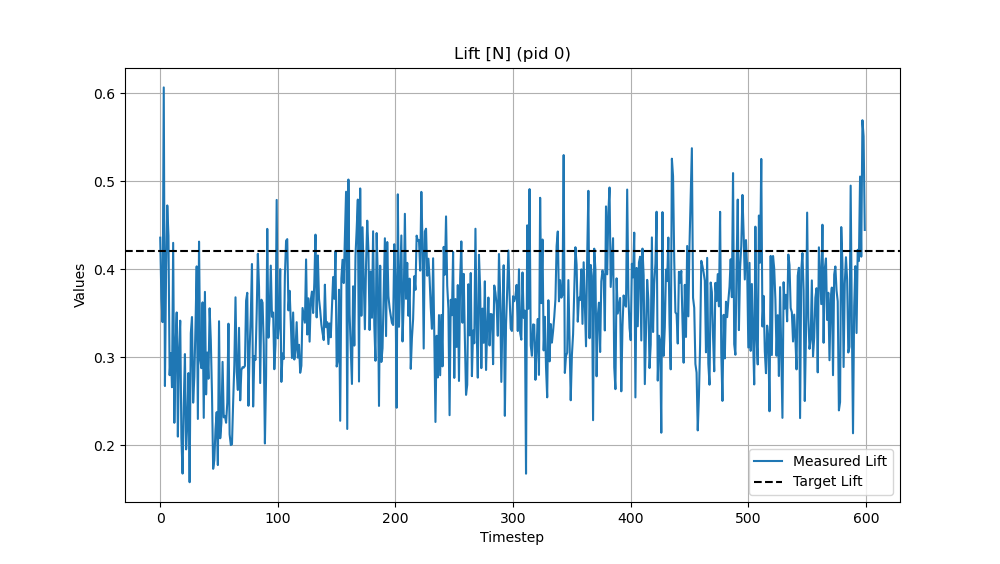
\includegraphics[width=\textwidth]{./img/LiftPID0.png}
        \caption{PID at $\SI{0}{\degree}$}
    \end{subfigure}
    \caption{Measured lift vs target for each model}
    \label{fig:measurement_lift}
\end{figure}

Pictured in Figure~\ref{fig:measurement_lift} are the resulting measurements for lift across each of the runs. While the MPC performs notably better than PID -- quickly converging close to the target lift -- performance lacks behind the DRL implementation. Figure~\ref{fig:measurement_lift-DRL} shows results for both TD3 and SAC implementations~\cite{5}, where measured lift appears near constant around the target. Noticeable dips in output are observable at timesteps 0 and 300, however this is a result of the measurement being performed across two training episodes, with random actuation of the motors at the beginning of each.
\\
\begin{figure}[h]
    \begin{center}
        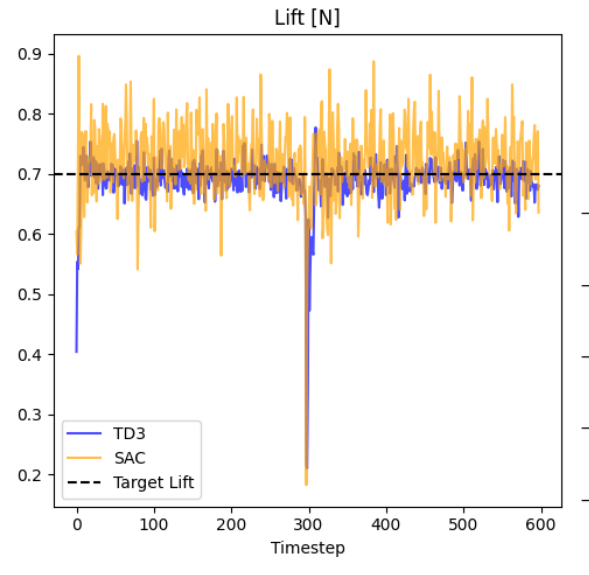
\includegraphics[width=0.5\textwidth]{./img/LiftDRL}
    \end{center}
    \caption{DRL lift response for 0.7N target~\cite{5}}\label{fig:measurement_lift-DRL}
\end{figure}
\\

Figure~\ref{fig:measurement_actuator-PID0} provides a plot for the actuator position over time during a PID run, with Figure~\ref{fig:measurement_actuator-PID0b} showing the final position of the wing. As evident by the graph, the controller in this run quickly moves to a position position of $1.0$ normalised at the beginning, maintaining this pose for the remaining duration. 

\begin{figure}[h]
    \begin{subfigure}[b]{0.53\textwidth}
        \centering
        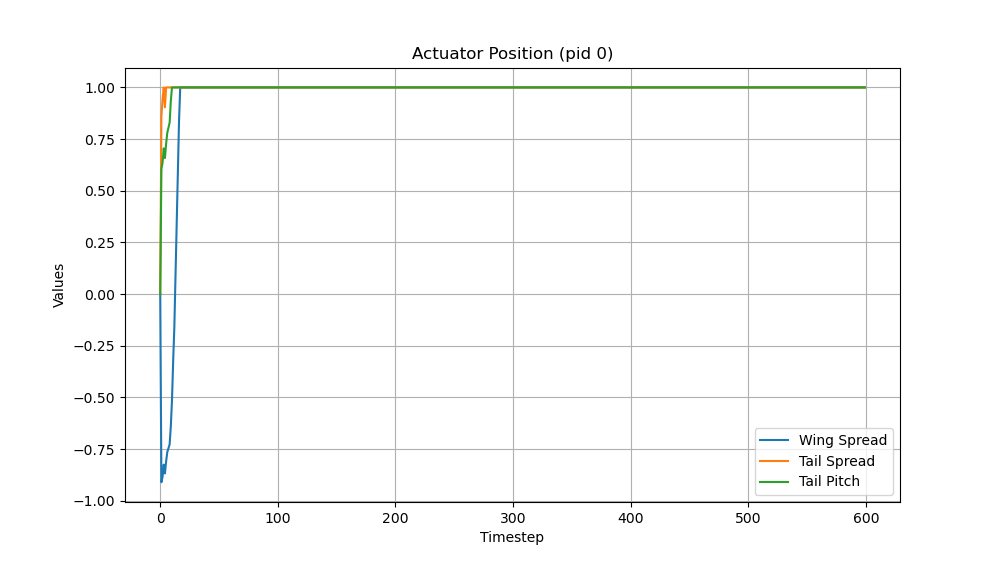
\includegraphics[width=\textwidth]{./img/ActuatorPID0.png}
        \caption{Actuator position}
    \end{subfigure}
    \begin{subfigure}[b]{0.45\textwidth}
        \centering
        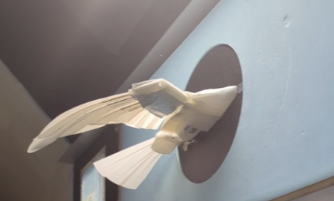
\includegraphics[width=\textwidth]{./img/wing_PID0.png}
        \caption{Final wing pose}\label{fig:measurement_actuator-PID0b}
    \end{subfigure}
    \caption{Actuator position and final pose for wing running PID at $\SI{0}{\degree}$}
    \label{fig:measurement_actuator-PID0}
\end{figure}\vspace{1em}

This contrasts with the resulting actuations of the DRL controllers, resulting in more motion to maintain stability of the lift at target. Final positions of the wing from the paper are shown in Figure~\ref{fig:wing_DRL}, where its clear the position deviates from what was observed with the PID implementation.

\begin{figure}[h]
    \begin{center}
        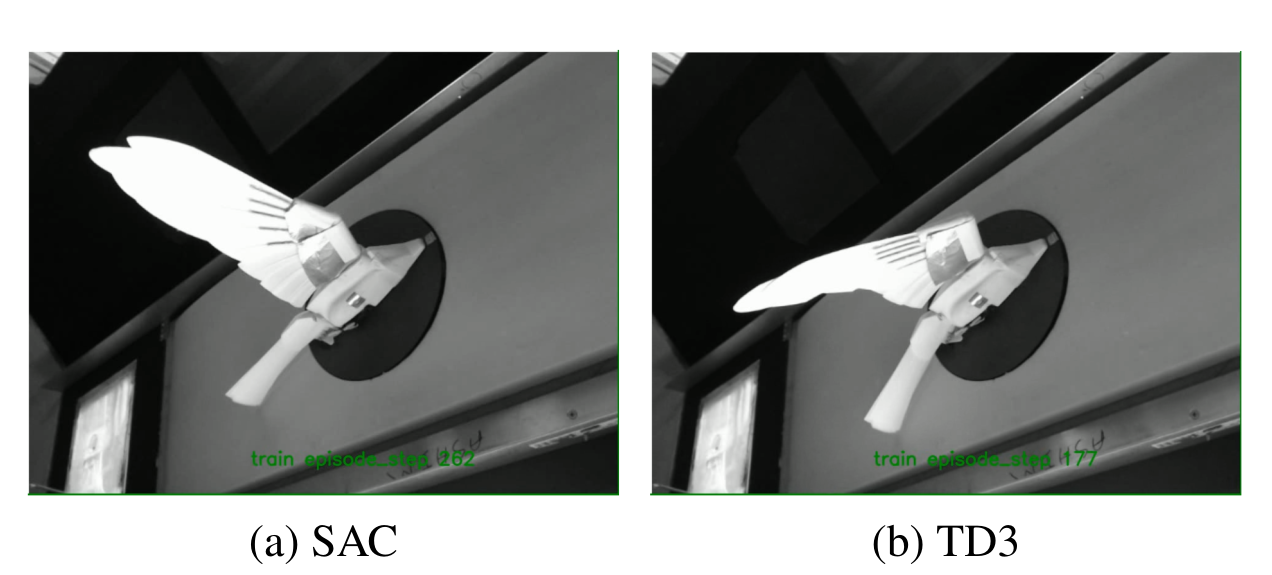
\includegraphics[width=0.8\textwidth]{./img/wing_DRL.png}
    \end{center}
    \caption{Final pose for wing running DRL}\label{fig:wing_DRL}
\end{figure}


\section{Discussion}
\section{Conclusion}
